%! TEX root = ./main.tex
% Rayleigh-Jeans

\subsubsection{傅里叶级数}%

\begin{figure}[h]
	\centering
	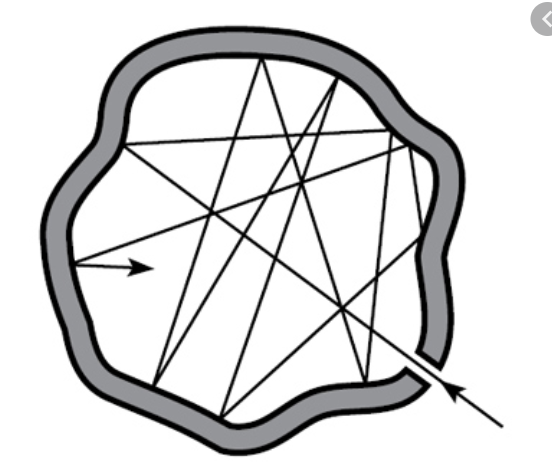
\includegraphics[width=0.2\linewidth]{figures/cavity.png}
	\caption{Cavity}%
	\label{fig:cavity}
\end{figure}

黑体辐射达到平衡后,源给场多少能量,场也给源多少能量。
由源产生的电磁波满足波动方程
\begin{equation}
	\label{eq:wave_eq}
	\laplacian{\psi} - \frac{1}{c^2} \pdv[2]{\psi}{t}=0
\end{equation}

\begin{note}
没有人会去背这个方程,因为这个方程其实就是对闵科夫斯基空间的四个基矢$[x,y,z,ict]$的二阶偏导:
\[
	\left(\pdv[2]{x} +\pdv[2]{y} +\pdv[2]{z} +\pdv[2]{ict} \right)\psi = 0
\]
\end{note}

方程\eqref{eq:wave_eq}的通解就等于特解的线性叠加。

任何一组连续振动的体系都等效于一组谐振子。
任何电磁波都能分解为单色波的叠加。
黑体辐射的能量密度,可以由无数个简谐振子组成。
实际上,这个辐射源就等效于一组谐振子,这些谐振子有不同的频率,就出来不同频率的平面波,把他们叠加,就出来了电磁场。

我们用一个尝试解带入:
\begin{equation}
	\begin{aligned}
		\label{eq:superposition}
			\Psi = \sum_{k} \psi_k  \\
			\psi_k(x,y,z,t)=q_k(t)\exponential(ik\vdot r)
	\end{aligned}
\end{equation}

\begin{align*}
	\sum_{k} \left[ q_k(t) \laplacian \exp(ik\vdot r) - \frac{1}{c^2} \exp(ik \vdot r) \ddot{q_k}(t) \right] = 0 \\
	\laplacian{\exp(i\vb{k}\vdot\vb{r})} = - k^2 \exp(i\vb{k}\vdot\vb{r}) \\ 
	\ddot{q_k}(t)+c^2 k^2 q_k(t) = 0\\
	\omega^k=ck= \frac{2\pi}{\lambda}c=2\pi \nu_k\\
	q_k(t)=A\exp(-i \omega_k t)
\end{align*}

解得

\begin{equation}
	\psi_k(x,y,z,t)=A\exp[ -i(\omega_k t-\vb{k}\vb{r}) ]
\end{equation}


\subsubsection{箱归一化}%

这个解是在没有边界的情况得出的,若有边界应该怎么办呢:
% TODO 加黑体辐射空腔图

假设周期性边界条件:

\begin{subequations}
	\begin{align}
		\psi(x,y,z,t) = \psi(x+L,y,z,t)\\
		\psi(x,y,z,t) = \psi(x,y+L,z,t)\\
		\psi(x,y,z,t) = \psi(x,y,z+L,t)
	\end{align}
\end{subequations}
\begin{subequations}
	\begin{align}
	e^{i k_x L} = 1\\
	e^{i k_y L} = 1\\
	e^{i k_z L} = 1
	\end{align}
\end{subequations}
\begin{subequations}
	\begin{align}
		k_x L = 2\pi n_x \quad k_x=\frac{2\pi}{L}n_x  \quad (n_x=0,\pm 1,\pm 2, \ldots)\\
		k_y L = 2\pi n_y \quad k_y=\frac{2\pi}{L}n_y  \quad (n_y=0,\pm 1,\pm 2, \ldots)\\
		k_z L = 2\pi n_z \quad k_z=\frac{2\pi}{L}n_z  \quad (n_z=0,\pm 1,\pm 2, \ldots)
	\end{align}
\end{subequations}
\begin{equation*}
	\omega_k=2\pi \nu_k = c|\vb{k}| = \frac{2\pi}{L}c\sqrt{n_x^2+n_y^2+n_z^2} 
\end{equation*}
%TODO k 空间到 n 空间的配图

从$n$空间到$k$空间只相差了一个系数,设这个系数为 $\lambda$, 即$\lambda = \left(\frac{L}{2 \pi}\right)^3 = \frac{V}{\left(2 \pi\right)^3}$。现在随便划出一个体积 $\Delta V=\Delta n_x \Delta n_y \Delta n_z$,里面的状态数在数值上就等于n空间的体积:
\begin{equation}
	\begin{aligned}
		\label{eq:space}
		\text{状态数} &=  \Delta n_x \Delta n_y \Delta n_z \\
		&= \lambda \Delta k_x \Delta k_y \Delta k_z \\
		&=   \frac{L}{2 \pi} ^3 \Delta k_x \Delta k_y \Delta k_z  \\
		&=   \frac{V}{{\left( 2 \pi \right)}^3} \Delta k_x \Delta k_y \Delta k_z
	\end{aligned}
\end{equation}

数出在 $\abs{\vectorbold{k}} \sim \abs{\vectorbold{k}} + \dd \abs{\vectorbold{k}}$ 的状态数,只要算出 k 空间球壳的体积,再乘 $\lambda$

笛卡尔坐标转换为球坐标, 并考虑到电磁波的两种独立的偏振,需要乘2

\begin{equation}
	Z_k \dd k = \lambda \cdot \dd k \int_{0 }^{\pi } \sin\theta \dd{\theta}   \int_{0 }^{2\pi } \dd{\phi}  = \lambda \cdot 4 \pi k^2 \cdot \dd k = \frac{V}{(2 \pi)^3} \cdot 4 \pi k^2 \cdot \dd k
\end{equation}

$|\vb{k}| \to \omega $ $(k=\frac{\omega}{c})$
\begin{equation}
	Z'_k d\omega = \frac{4 \pi V}{(2 \pi)^3} \left(\frac{\omega}{c}\right)^2 \dd{\left(\frac{\omega}{c}\right)}  = \frac{4 \pi V}{(2 \pi )^{3}} \frac{\omega^2 d\omega}{c^3}
\end{equation}

\begin{equation*}
	Z_\omega \dd\omega = \frac{V \pi \omega^2 \dd\omega}{(2 \pi c)^3}
\end{equation*}

$ \omega \to \nu $ ($\omega = 2 \pi \nu$)
\begin{equation*}
	Z_\nu \dd \nu = \frac{V}{c^3} 8 \pi \nu^2 \dd \nu
\end{equation*}

设频率在 $\nu \sim \nu + \dd \nu$ 区间的态密度为 $\rho_\nu$
\begin{equation*}
	\rho_\nu = Z_\nu = \frac{V}{c^3} 8 \pi \nu^2 
\end{equation*}

其能量:
\begin{equation}
	\label{eq:Density_of_States}
	\rho_\nu \dd \nu \overline{\varepsilon_\nu}= \frac{8 \pi \nu^2}{c^3} \dd \nu \vdot \overline{\varepsilon_\nu}
\end{equation}

能均分定理。假设:能量是连续的,能量是动量的连续函数,求和变成积分\footnote{要真正解决这个问题,需要普朗克能量量子化,需要能量是频率的函数, 盲猜,什么函数最容易,正比最容易,所以先猜 $E(\nu)=h\nu$,类比傅里叶级数的振幅?这是后话。}:


\begin{equation}
	\label{eq:equipartition_theorem_of_energy}
	\overline{\varepsilon_\nu} = \frac{\overline{p^2} }{2m} + \overline{\frac{1}{2}m\omega^2q^2} = kT
\end{equation}

把方程\eqref{eq:equipartition_theorem_of_energy}带入方程\eqref{eq:Density_of_States}  得

\begin{equation}
	\rho_\nu \dd\nu = \frac{8 \pi \nu^2}{c^3} kT \dd \nu
\end{equation}

